\subsection{Lab6: Interfaces gráficas de  WX GUI}
%*********************
\begin{frame}{}

\pgfdeclareimage[width=\paperwidth,height=\paperheight]{bg}{imagenes/fondo_lab}
\setbeamertemplate{background}{\pgfuseimage{bg}}

\bfseries{\textrm{\LARGE Interfaces gráficas con \newline WX GUI}}
\raggedright
\end{frame}
%*********************

\begin{frame}{Grid position}

\pgfdeclareimage[width=\paperwidth,height=\paperheight]{bg}{imagenes/fondo3}
\setbeamertemplate{background}{\pgfuseimage{bg}}

\textbf {Posicionamiento de rejilla} \\
\vspace{2mm}
GRC ofrece varios receptores gráficos y controles gráficos para crear gráficos de flujo wx-gui.(scope sink, fft sink, number sink, waterfall sink, constellation sink, slider control, and chooser control) Cada uno de estos elementos gráficos tiene un parámetro de posición de cuadrícula para un posicionamiento preciso.

\end{frame}
%-----------------------------------

\begin{frame}{Grid position}

\begin{figure}[H]
\centering
\vspace{-3mm}
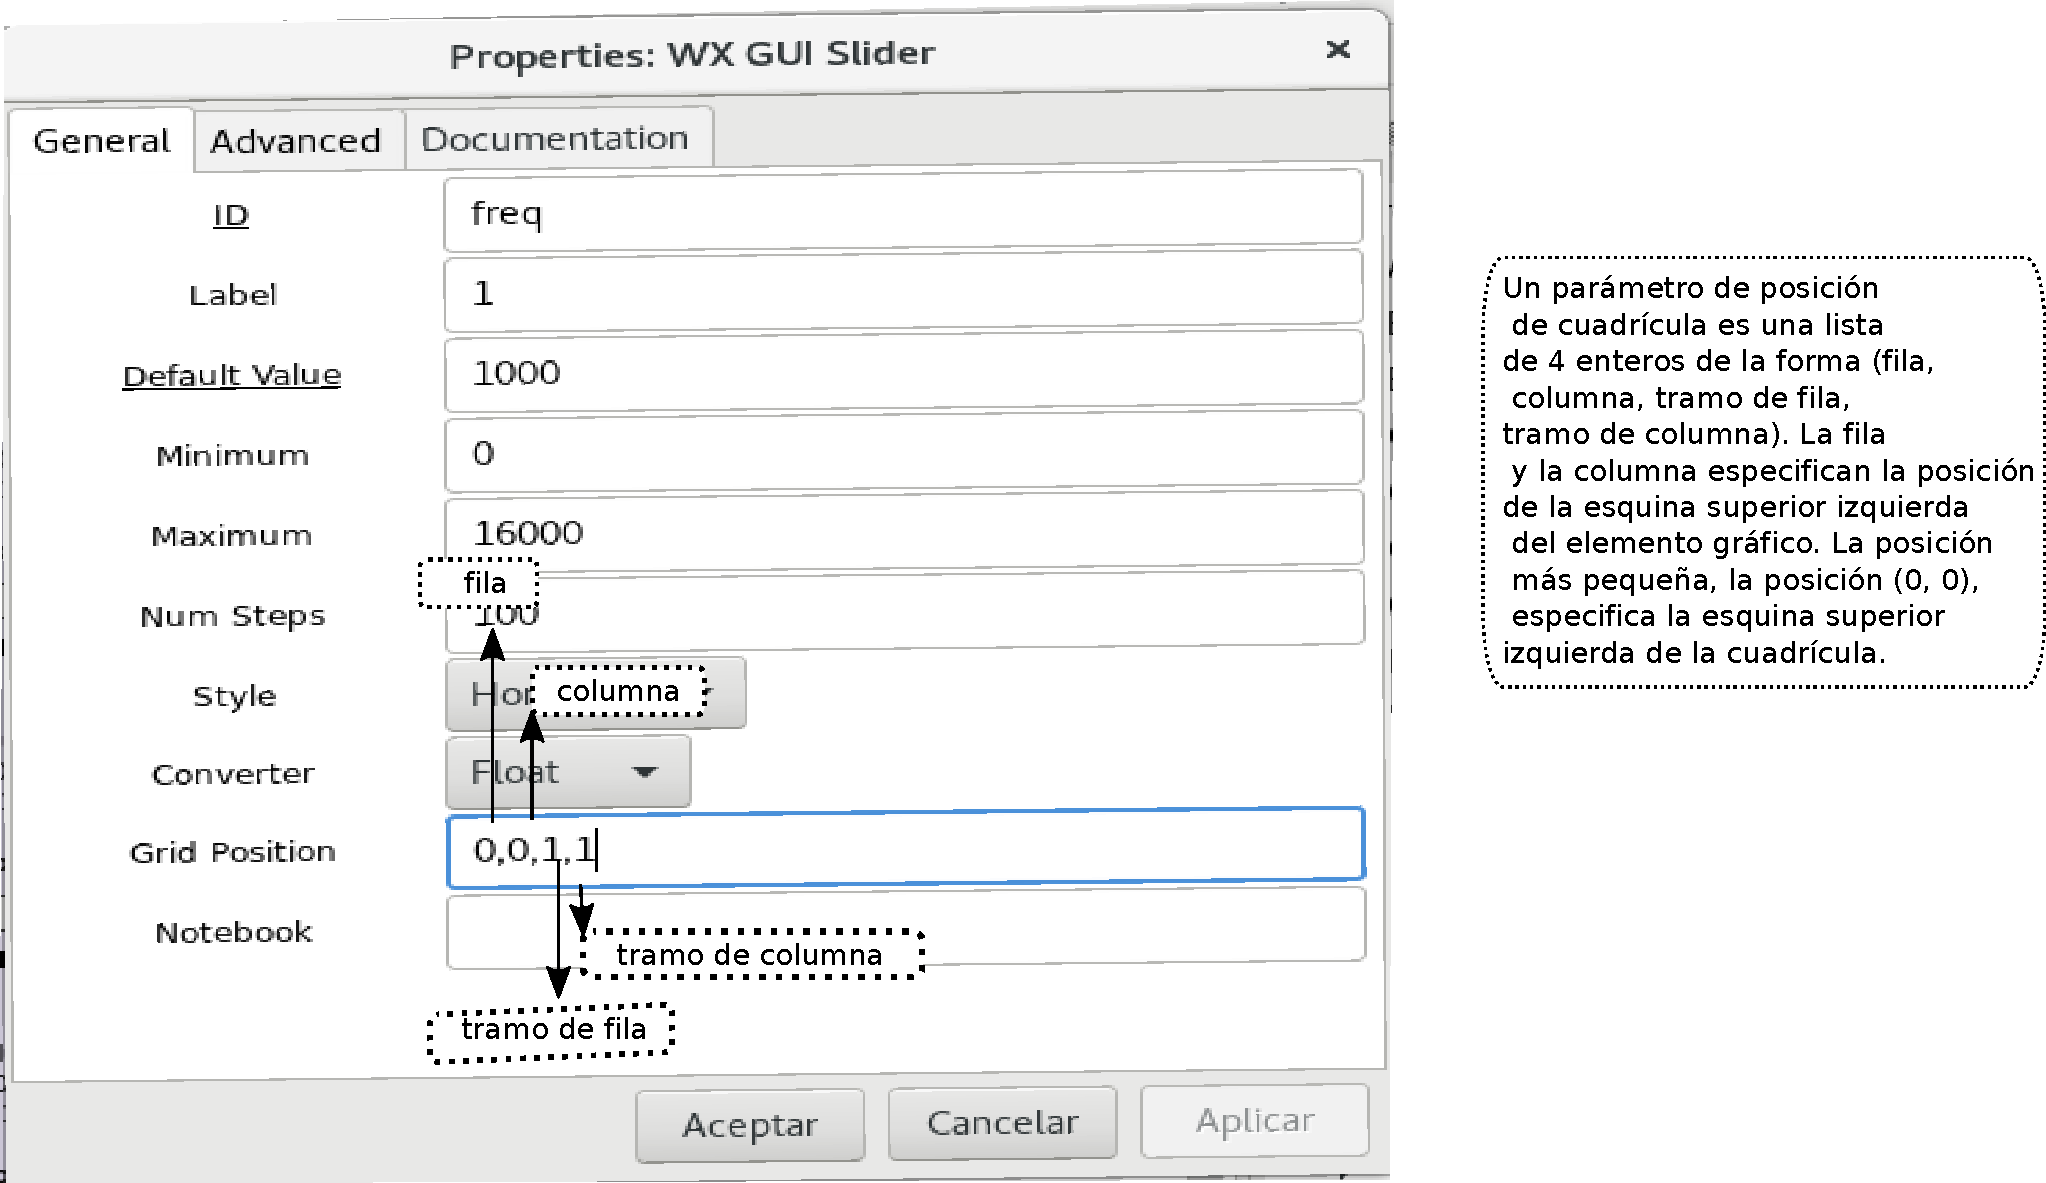
\includegraphics[width=0.9\textwidth]{parte1/lab00/pdf/lab0_1.pdf}


\end{figure}

\end{frame}
%-----------------------------------

\begin{frame}{Grid position}

El tramo de fila especifica el número de filas hacia abajo desde la posición de la fila, y el tramo de columna especifica el número de columnas a la derecha de la posición de la columna. Por lo tanto, el tramo debe ser al menos (1, 1) para ocupar el mínimo de 1 celda de cuadrícula.

\end{frame}
%-----------------------------------

\begin{frame}{Grid position}

\begin{figure}[H]
\centering
\vspace{-3mm}
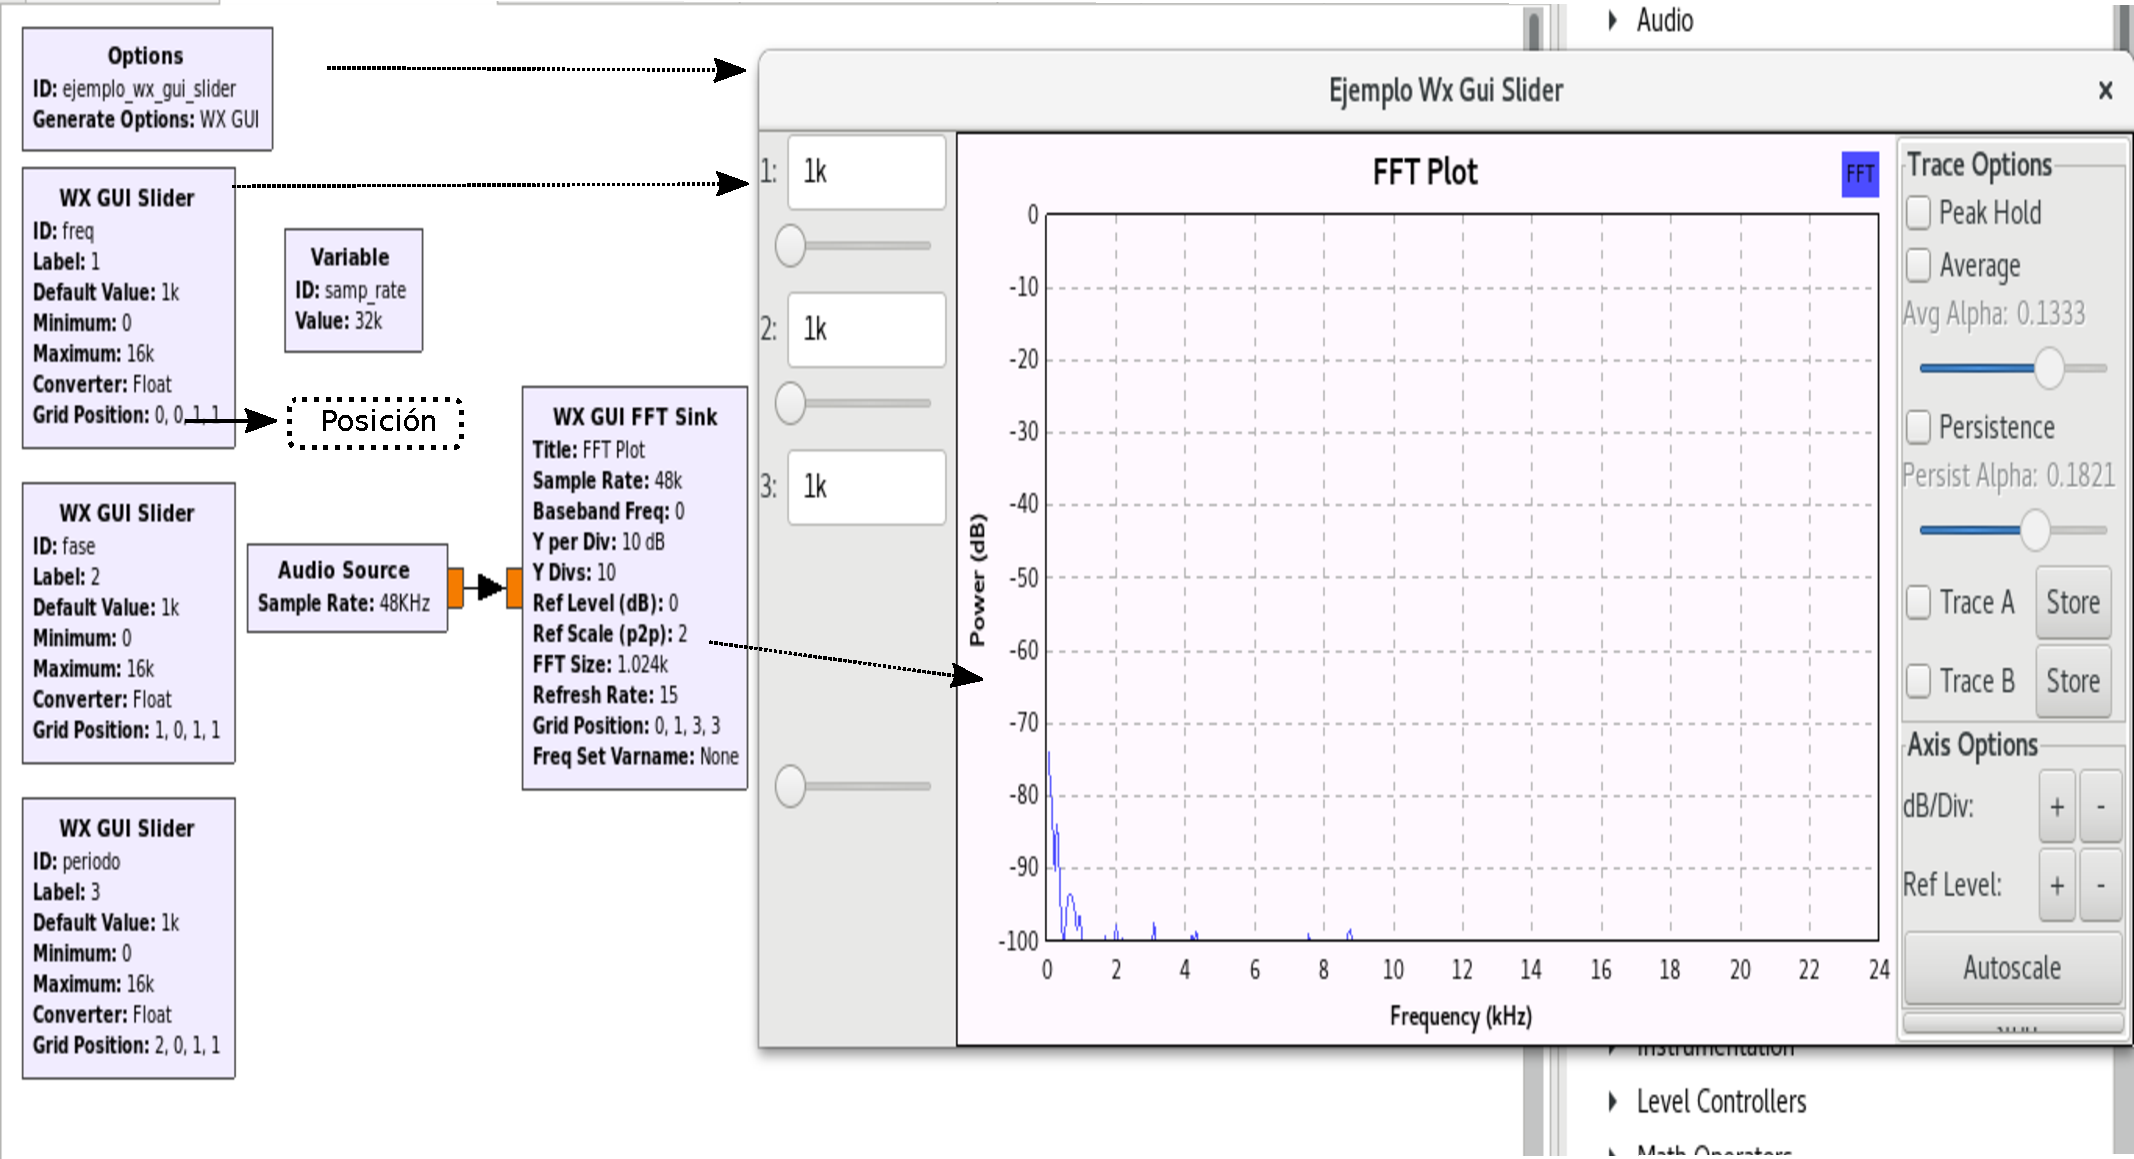
\includegraphics[width=0.9\textwidth]{parte1/lab00/pdf/lab0_2.pdf}
\end{figure}

\end{frame}
%-----------------------------------

\begin{frame}{Grid position}

\begin{figure}[H]
\centering
\vspace{-3mm}
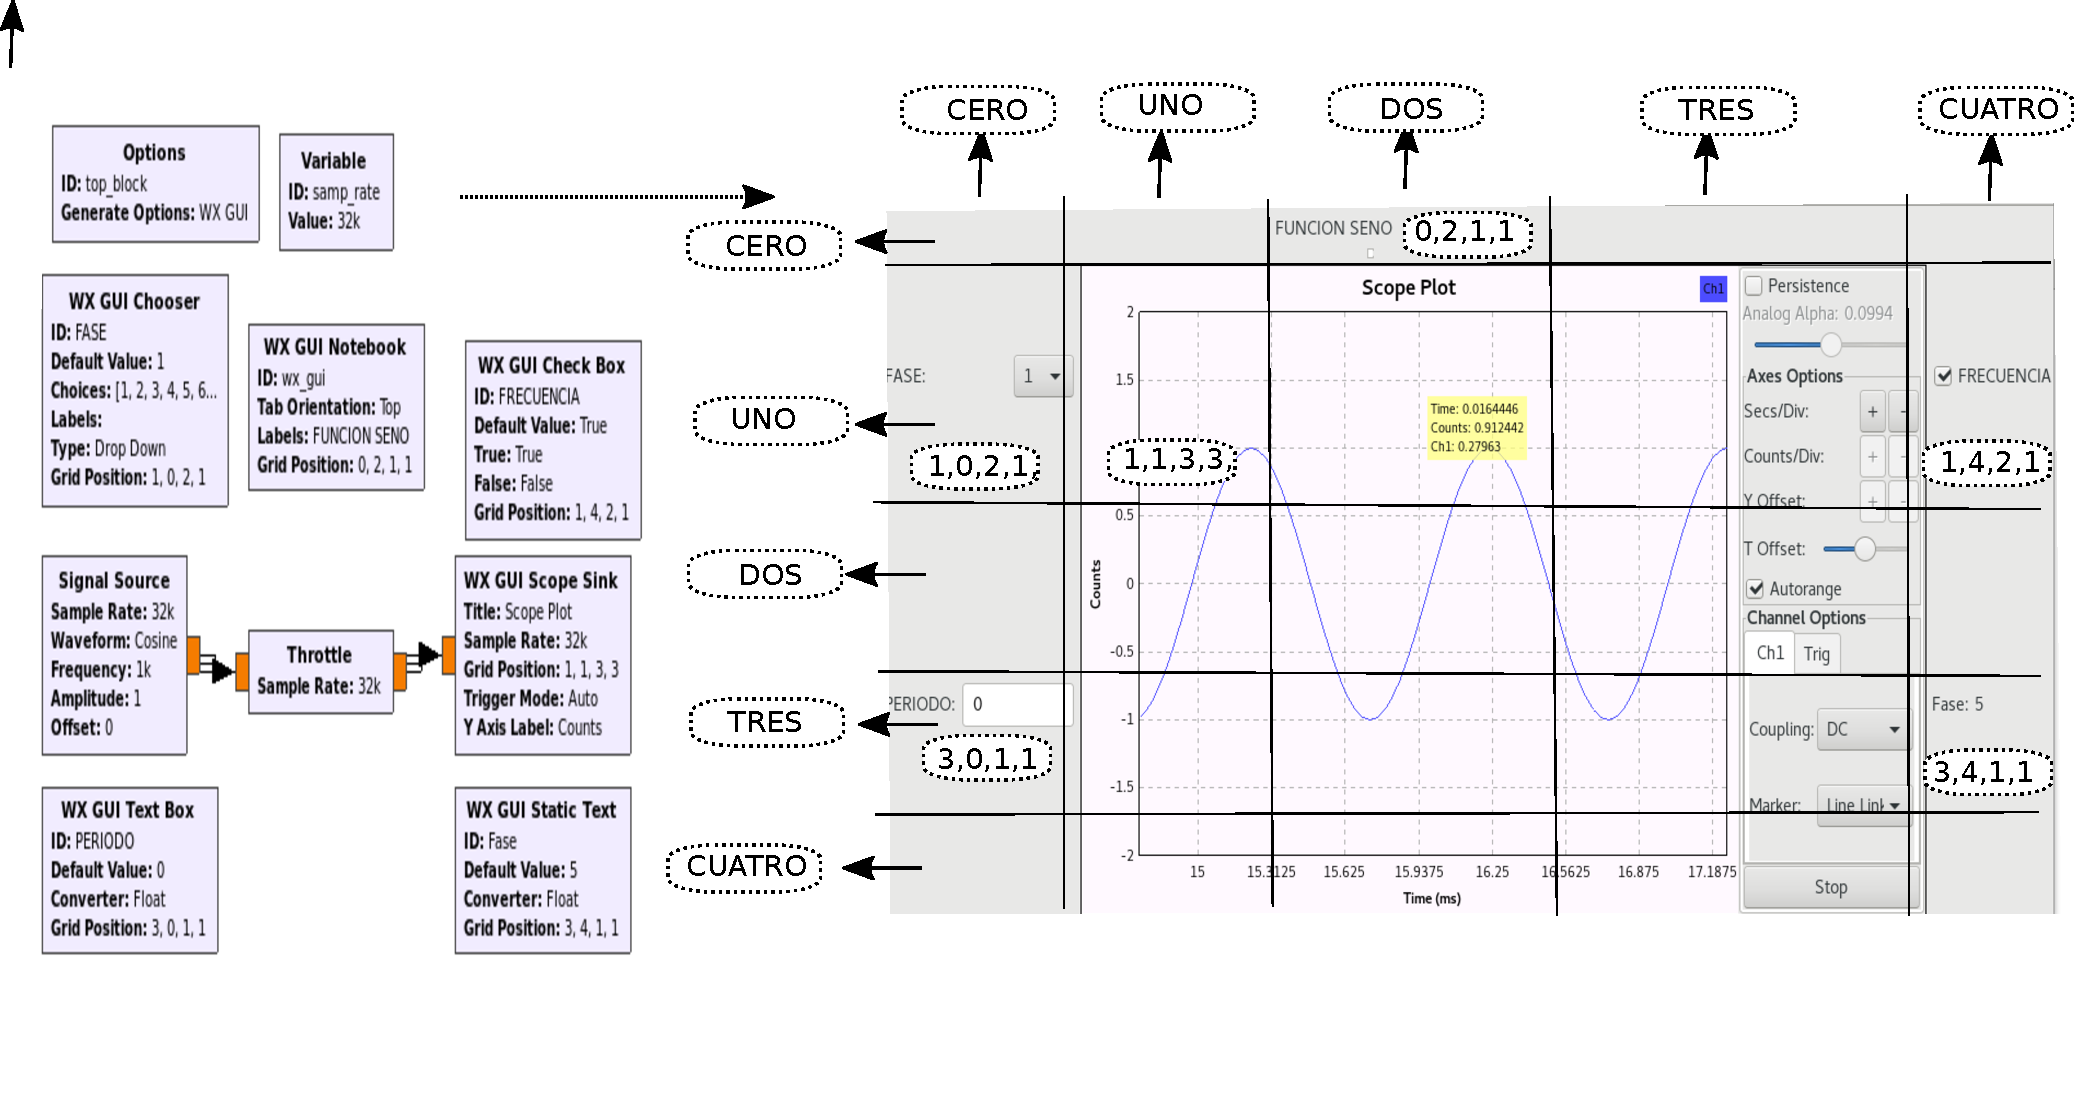
\includegraphics[width=0.9\textwidth]{parte1/lab00/pdf/lab0_3.pdf}
\end{figure}

\end{frame}
%-----------------------------------
